\chapter{Theoretical Background} \label{sec:theo}
This chapter will introduce the fundamentals necessary to understand the following chapters. The first section will define the coordinate systems used in this thesis.
Next point clouds are introduced  and algorithms and sensors for generating them are presented.
The following section will present an efficient connected components labeling algorithm.
The next section explains artificial neural networks and \acp{cnn}.
In the last section the \ac{pca} is introduced.

\section{Coordinate Systems} 
\subsection{Vehicle Coordinate System} \label{sec:theo:vehicleCoord}
According to ISO 8855 \cite{ISO8855} 
a vehicle axis system is defined with the $x$-axis pointing horizontally forward. 
The $y$-axis is horizontal as well, pointing left with respect to the forward direction. The $z$-axis points upwards, so that it forms a right handed trihedron. The rotation around the $x$-axis is referred to as roll, the rotation around the $y$-axis as pitch and the rotation around the $z$-axis as yaw or heading.
The vehicle coordinate system is defined by the vehicle axis system and the vehicle reference point, that is the origin of the coordinate system.

If not stated otherwise this work will use this coordinate system with the vehicle reference point located in the centre of the camera.

\begin{figure}[h!]
    \centering
    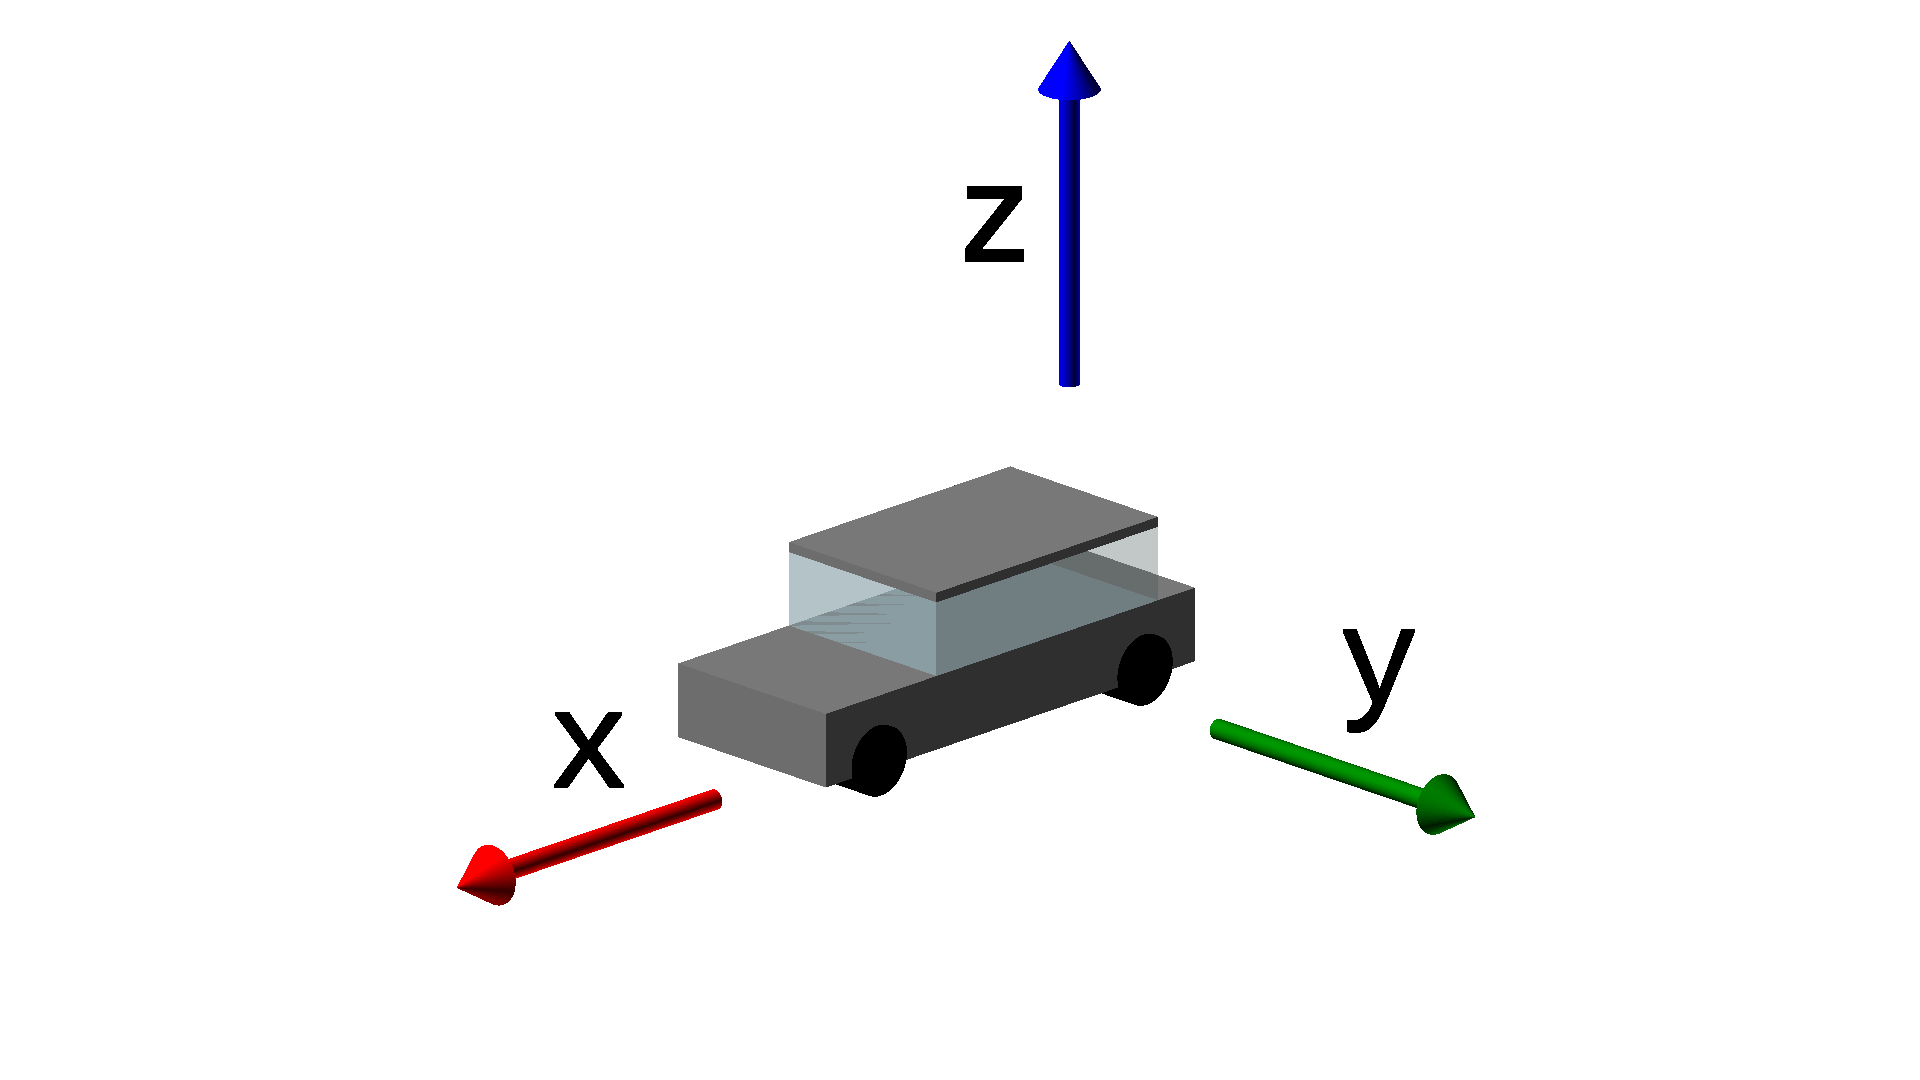
\includegraphics[width=\textwidth]{coord.png}
    \caption{Vehicle Coordinate System (Source: Own illustration)}
    \label{fig:theo:coord}
\end{figure}

\subsection{Image Coordinate System} \label{sec:theo:imageCoord}
For images the coordinate system consists of a $x$-axis pointing right and a $y$-axis pointing downward. The origin of the coordinate system is in the top left of the image.

\begin{figure}[h!]
    \centering
    \begin{tikzpicture}[scale=0.5]
        \pgfmathtruncatemacro{\scale}{1}
        \foreach \x in {0,1,...,9}{
            \foreach \y in {0,1,...,9}{
                \pgfmathtruncatemacro{\xpos}{\x * \scale};
                \pgfmathtruncatemacro{\ypos}{\y * \scale};
                \filldraw [draw=black,fill=gray!40] (\xpos,\ypos) rectangle (\xpos+\scale,\ypos+\scale);
            }
        }
        \draw[line width=3pt,arrows={-triangle 60}] (-1,10) -- (-1,0);
        \node (y) at (-2,5){$y$}; 
        \draw[line width=3pt,arrows={-triangle 60}] (0,11) -- (10,11);
        \node (x) at (5,12){$x$}; 
        
    \end{tikzpicture}
    \caption{Image Coordinate System (Source: Own illustration)}
\end{figure}

\section{Point Clouds}
A point cloud is a set of points in space, that is usually the $\mathbb{R}^3$. A point cloud is either created artificially or more commonly captured by a sensor, in
this case the point cloud gets sampled from a 3D object \cite{pclAbout}.

\begin{figure}[h!]
    \centering
    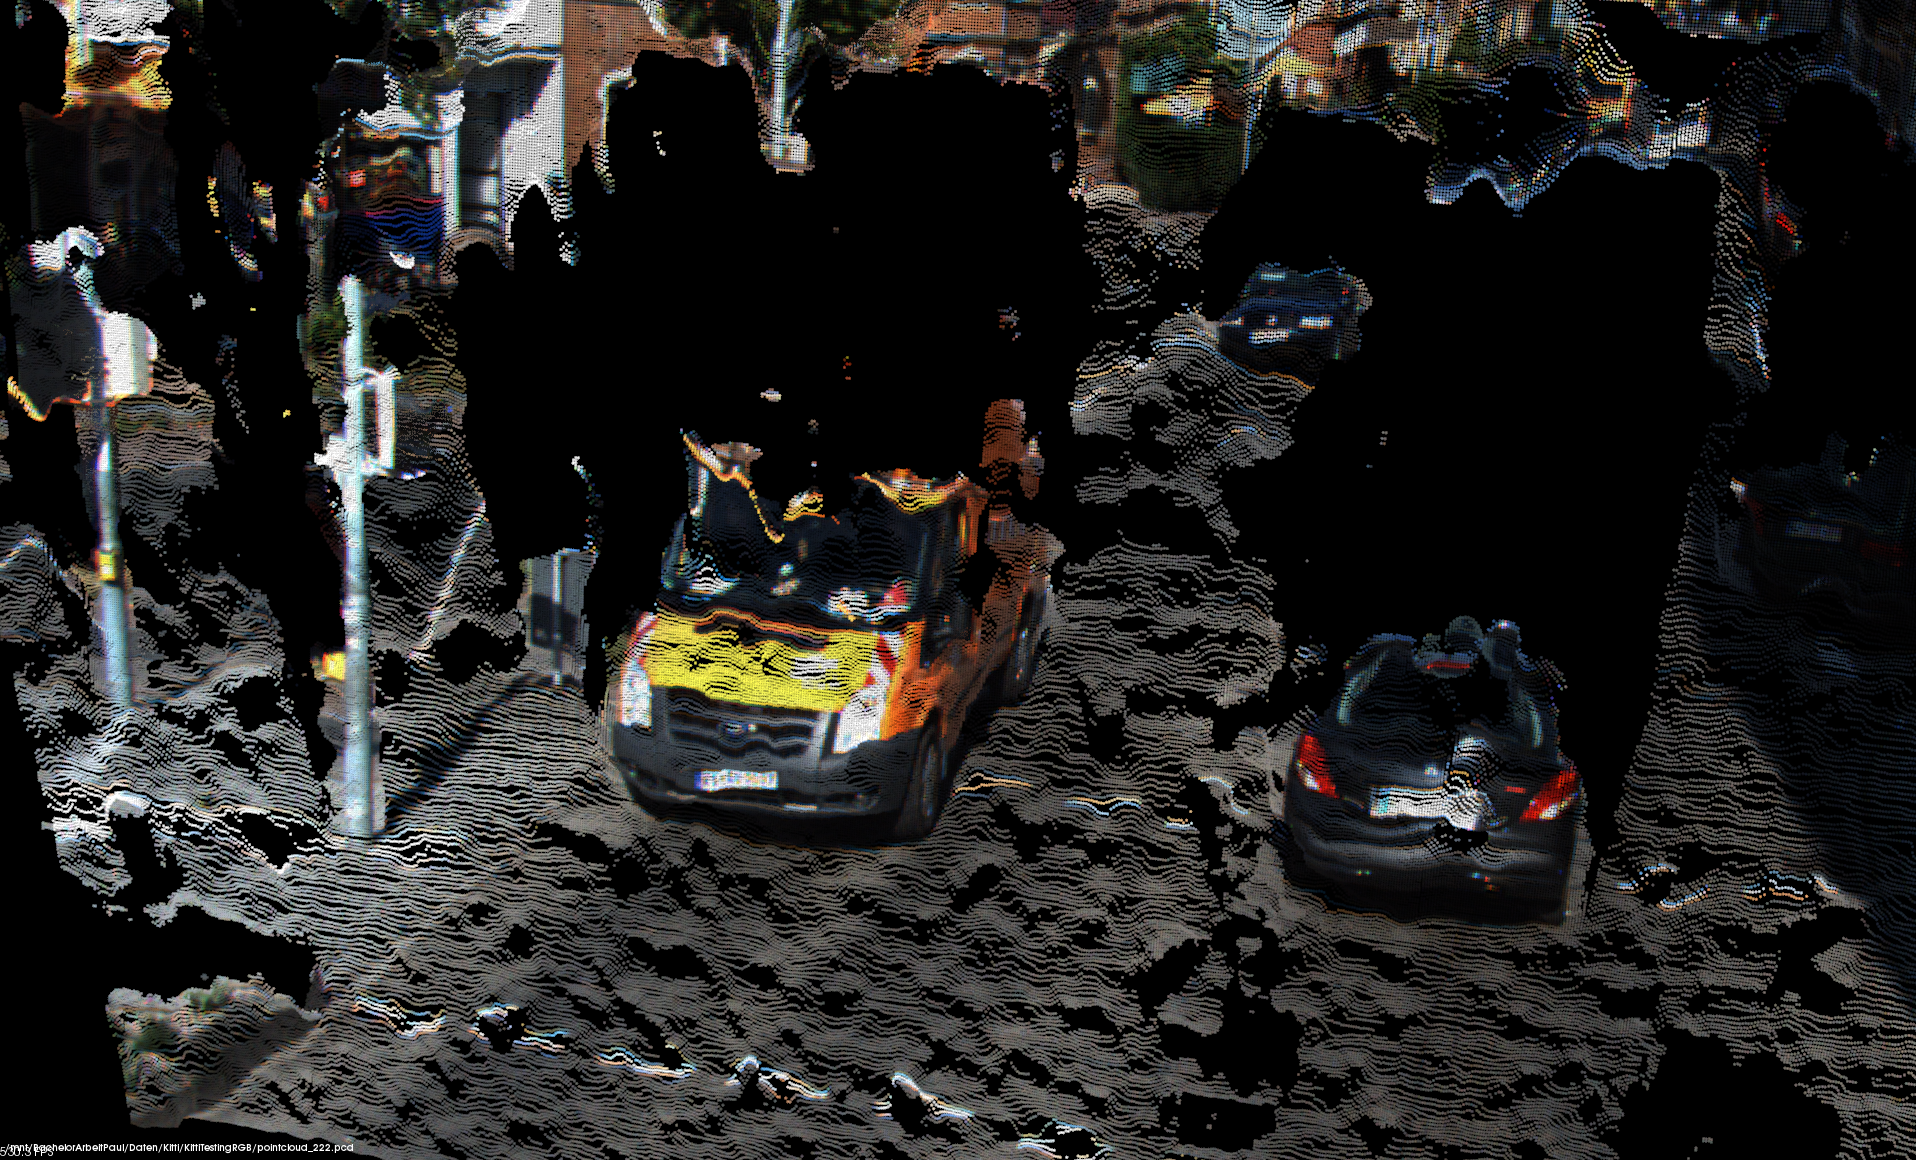
\includegraphics[width=\textwidth]{../Material/pointcloud.png}
    \caption{Example of a point cloud with additional colour information}
    \label{fig:theo:pc}
\end{figure}

Each point in a point cloud is usually represented by a vector consisting of the $x$, $y$ and $z$ coordinate. In addition to the coordinates more information can be stored for every point. Commonly used values are the reflectivity, surface normals or the colour of each point. 

Figure \ref{fig:theo:pc} shows a point cloud which depicts an urban scene,
the point cloud is generated from the Kitti dataset \cite{Menze2015CVPR}.
In addition to the points in space there is also colour information for every point.
This additional colour information is often referred to as texture \cite{pclAbout}.

\subsection{Stereo Vision}
By taking pictures from a scene from two positions it is possible to calculate distance information from the scene by exploiting the difference between the images \cite{stereoHaw10}.
This process is called stereo vision and is similar to what the human brain does with the information of two eyes. 

In general, stereo vision is based on matching a pixel found in one of the images to a pixel in the second image. 
The distance between the two positions of the pixels is called disparity, which is inverse proportional to the actual distance of the point. 
By combining the disparity for every pixel into an image at the corresponding position a disparity image or disparity map is created.

\begin{figure}[h!]
    \centering
    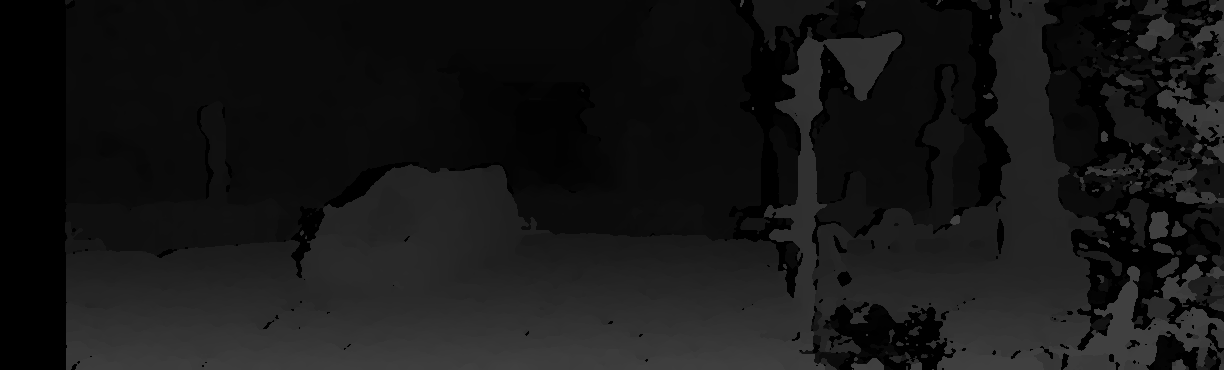
\includegraphics[width=\textwidth]{disparity.png}
    \caption{Example of a disparity map }
    \label{fig:theo:disp}
\end{figure}

Figure \ref{fig:theo:disp} shows a disparity map generated from the Kitti dataset \cite{Menze2015CVPR}, the disparity values are mapped onto different colours, with orange being large disparities and blue small disparities.

In the following sections two algorithms for the calculation of disparity maps are presented.

\subsubsection{Rectification}
For a pixel in one of the images all possible points in the real world are located on a line \cite{stereoHaw10}.
In the second image this set of points is visible as a line, which is called the epipolar line. 
As all pixels that can possible correspond to a pixel in the first image lie on the epipolar line on the second image it is sufficient to only search for matches on this line.
To simplify the matching it is beneficial for the epipolar line to be straight and horizontal.
This is achieved by rectifying the image, that is transforming the images, such that all epipolar lines are horizontal. This results in transformed images which appear to be taken with two cameras with only horizontal displacement and no relative rotation.

\begin{figure}[h!]
    \centering
    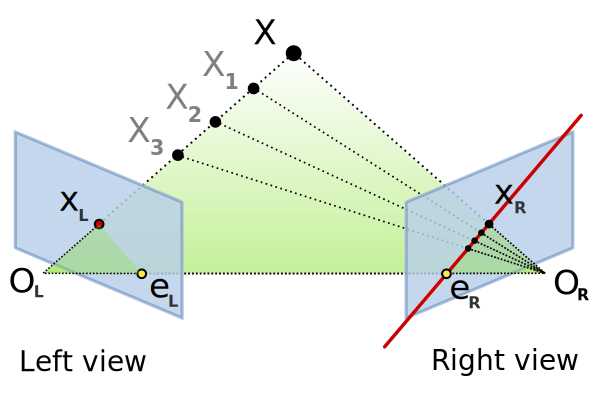
\includegraphics[width=\textwidth]{EpipolarGeometry.pdf}
    \caption{Point as part of the epipolar line (Source: Arne Nordmann [cc by-sa 3.0])}
    \label{fig:theo:epipolarLine}
\end{figure}

Figure \ref{fig:theo:epipolarLine} shows the views of a stereo system with the left camera, positioned at $O_L$, and the right camera positioned at $O_R$. 
All points $X$, $X_1$, $X_2$ and $X_3$ are located on a straight line and are projected to the same pixel $X_L$ in the left image. 
In the right image the points are located on a straight line, this line can be seen as the red line. 
All possible matches $X_R$ for the pixel $X_L$ are located on this epipolar line.
As the epipolar line is not horizontal the images require rectification.

Rectification is done by linear transforming the images. For this a transformation matrix $H$, so that an image point $p$ is transformed into $\vec{p}$ need to found.

\subsubsection{Semi-Global Matching} \label{sec:theo:sgm}
Semi-Global Matching \cite{Hirsch05} \cite{sgm2} is one the most commonly used \cite{stereoHaw10} algorithms for calculating disparity maps, primarily based on the fact that it is able to run in real time  while still producing precise results \cite{middleburyStereo3}. 
The algorithm performs dense stereo matching, this implies that for nearly every pixel a corresponding pixel is found. 
The algorithm combines the advantages in computational performance of pixel wise matching with the advantages in quality of a global cost function, which considers the complete image for matching.

The global cost function is accumulated over eight directions: both vertical directions, and horizontal directions and the diagonal directions. For every direction the cost function is calculated independently.

The cost function is calculated by scanning the image along the respective directions. 
This reduces the problem from a two dimensional problem to multiple one dimensional problems on a scanline \cite{sgmHeidelberg}.

Along this scanline a similarity function $C: (p,d) \to \mathbb{R}$ is calculated. This function represents the similarity of a pixel $p$ to a pixel $\tilde{p}$ with disparity $d$. 
This similarity can be calculated by comparing the intensity at the position $p$ with the intensity at the pixel $\tilde{p}$.
This second pixel is the pixel on the epipolar line with a distance of $d$ from $p$.
The algorithm selects a disparity for every pixel. As the pixels next to each other are not independent of each other the similarity of the disparity, that is the smoothness of the resulting disparity map, should be enforced. 
For this a loss function $L_\text{Direction}(p,d)$ considering the neighbouring pixels is defined, using the constants $P_1$ and $P_2$ as non smoothness penalty:
\begin{eqnarray}
    n_i &=& L_\text{Direction}(p-1,d+i) \\
    L_\text{Direction}(p,d) &=& C(p,d) + \min\{n_0, n_1 + P_1, n_{-1} + P_1, \min_i (n_i) + P_2\}
\end{eqnarray}
The loss is calculated twice along the scanline, first in a forward pass and secondly backwards along the scanline. For every pixel a loss over all directions is calculated as the sum of the losses in the different directions:
\begin{equation}
    L_\text{Overall}(p,d) = \sum_{\text{Direction} \in \text{All Directions}} L_\text{Direction}(p,d)
\end{equation}

Using the overall loss for every pixel the disparity $d$ for a pixel $p$ can now be calculated as the disparity with the lowest loss, to speed up the computation a maximum disparity $d_\text{max}$ is used:
\begin{equation}
    d(p) = \text{argmin}_{d \in \{0, \ldots, d_\text{max} \} } \left(L_\text{Overall}(p,d)\right)
\end{equation}

% https://www.reddit.com/r/computervision/comments/9119qc/can_i_have_a_pseudo_code_explanation_of_the/

%http://lunokhod.org/?p=1356

\subsubsection{Calculating point clouds from Disparity Maps} \label{sec:theor:disp2pc}
Given the parameters of the individual cameras such as the focal length, and the parameters of the stereo system such as the translation and rotation between the two vantage points it is possible to compute the real world distances and as a result positions of pixels relative to the camera \cite{opencvpc}. 
Taking all these pixels as points in three dimensional space a point cloud can be calculated.
By additionally mapping the colour of each pixel onto the corresponding point a texture for the point cloud can be calculated.

Given the disparity $d(x,y)$ at a pixel ${(x,y)}^\text{T}$ and the corresponding calibration matrix $Q$ for the stereo system the position of the point in 3D space can be calculated:
\begin{eqnarray}
    \begin{pmatrix} 
        X \\ Y \\ Z \\ W
    \end{pmatrix}
    &=& Q \cdot 
    \begin{pmatrix}
        x \\ y \\ d(x,y) \\ 1
    \end{pmatrix} \\
    \vec{p}_\text{real world} &=& 
    \frac{1}{W}
    \begin{pmatrix}
        X \\ Y \\ Z
    \end{pmatrix}
\end{eqnarray}

\subsubsection{Depth Error Estimate} \label{sec:theo:error}
For many applications it is desirable to estimate the error of the depth measurement of a stereo system.
The depth error can be estimated given the distance $d$ to the object, the baseline $b$ that is the distance between the cameras, the focal length $f$ of the cameras and pixel matching error $\varepsilon_d$ \cite{stereoError}:
\begin{equation}
    \varepsilon \propto \frac{d^2}{b\cdot f} \cdot \varepsilon_d
\end{equation}

\subsection{Active Stereo Systems}
Passive vision based stereo systems have issues with textureless surfaces as no unambiguous correspondences can be found \cite{d435Structured}.
Additionally passive vision systems perform poor matching if the scene is not illuminated well.
To solve both issues an active system can be used. 
These systems use a projector to project an pattern onto the surface and thus provide a texture for every surface.
No a priori knowledge of the pattern or adaptation of the stereo matching algorithm is required \cite{d435Structured}.
To achieve unambiguous matches a non periodic pattern should be chosen, this can be done by using a semi-random pattern.

The \ac{d435} uses a projector which projects about 5000 points in a semi-random fashion using a laser projector \cite{d435Structured}.

%https://www.intelrealsense.com/wp-content/uploads/2019/03/WhitePaper\_on\_Projectors\_for\_RealSense\_D4xx\_1.0.pdf}
%https://www.intelrealsense.com/stereo-depth-vision-basics/}

\section{Connected Components Labeling} \label{sec:theo:concomp} 
Connected components labeling is used to find connected nodes in a graph.
Two nodes $n$ and $m$ of the same class are connected if there exists a path between them consisting entirely of nodes of their class \cite{digitalImageProcessing}.
The algorithm takes the graph as the input and returns for every class a set of nodes that belong to the class.

The algorithms for connected components labeling can be differentiated in one component at a time algorithms, which label objects separately \cite{abubaker2007}, and multipass algorithms which iterates over the nodes multiple times \cite{HeChaoSuzuki08}.

\cite{HeChaoSuzuki08} proposed an efficient two pass algorithm for connected components labeling.
The algorithm is designed to be used with images.
For images every pixel represents a node in the graph. 
The eight adjacent pixels of a pixel are the neighbouring nodes.
As the number of neighbours is bounded the algorithm runs in $\mathcal{O}(n)$ with $n$ being the number of pixels. 

The algorithm is explained in algorithm \ref{alg:theo:concomp}: first for every pixel a preliminary class is determined based on the neighbouring pixels, additionally equivalent classes are remembered. 
In the second step all identical classes are merged into the class with the lowest number.

% See: https://scicomp.stackexchange.com/questions/1429/dictionaries-in-pseudocode for dict
\begin{algorithm}[h!]
    \caption{Connected Components Labeling}\label{alg:theo:concomp}
    \begin{algorithmic}[1]
        \Procedure{ConnectedComponentsLabeling}{nodes}
            \State $\text{class} \gets -1 \text{ for every node} \in \text{nodes}$
            \State $\text{currClass} \gets 0$
            \State $\text{mappingToMinimal} \gets \text{empty dictionary}$
            \For {node $\in$ nodes} 
            \Comment{First pass: label all by neighbours, remember equivalent classes}
                \State equivalentClasses $\gets \emptyset$
                \For {neighbour $\in$ neighbours of node}
                    \If {$\text{sameClass}(\text{node}, \text{neighbour}) \land \text{class}[\text{neighbour}] >= 0$}
                        \State equivalentClasses $\gets \text{equivalentClasses} \cup \{\text{class}[\text{neighbour}]\}$
                    \EndIf
                \EndFor

                \If {equivalentClasses $= \emptyset$}
                    \State $\text{currClass} \gets \text{currClass} + 1$
                    \State $\text{class}[\text{node}] \gets \text{currClass}$
                \Else
                    \State $\text{minClass} = \gets \min(\text{equivalentClasses}$
                    \For {$\text{class} \in \text{equivalentClasses} \setminus \{\text{minClass}\}$}
                        \State $\text{mappingToMinimal}[\text{class}] = \text{minClass}$
                    \EndFor
                \EndIf
            \EndFor

            \For {node $\in$ nodes}
            \Comment{Second pass: merge equivalent classes}
                \While {$\text{class}[\text{node}] \in \text{mappingToMinimal}$}
                    \State $\text{class}[\text{node}] \gets \text{mappingToMinimal}[\text{class}[\text{node}]]$
                \EndWhile
            \EndFor
        \EndProcedure
    \end{algorithmic}
\end{algorithm}


\section{Artificial Neural Networks}
Artificial Neural Networks are algorithms, that mimic the human brain \cite{Hodgkin1952}. They consist of a set of neurons connected together as a graph. Each neuron takes a number of inputs, combines them with a given formula and produces an output, which is then propagated to the next neuron.
The parameters of the formula can be changed to adapt the output of the neural network.

For most neural networks there are two main phases \cite{bishop1995}: first learning, that is adapting the parameters to fit a certain function and forwarding, that is calculating the output for data the neural networks has not seen before.

There are three different paradigms for learning: unsupervised learning, which is used for tasks such as feature extraction and clustering, reinforcement learning, which is used if a reward can be defined but no ground truth data exists, and supervised learning which is used if labeled ground truth data exists. As this is the case for the neural network used in this thesis, only supervised learning will be explained in the following section.

In the following section first a simple neural network, the \ac{mlp} is explained.
Then the \acf{cnn} is explained as a special case of a \ac{mlp}.

\subsection{Neuron}
\cite{Hodgkin1952} modeled the activity of a neuron in the human brain with a continuous differential equation.
For larger neural networks this differential equation gets to complicated.
Thus the model has been simplified \cite{bishop1995}: The output is determined by calculating the weighted sum of all inputs $x_k$ and adding a so called bias $b$.
To be able to approximate nonlinear functions a nonlinear transfer function $f$ is then applied for every neuron:

\begin{equation}
    y = f\left(b + \sum_{k=1}^n x_k \cdot w_k \right)
\end{equation}

The structure of a neuron can be seen in Figure \ref{fig:theo:neuron}, the inputs $x_1$ to $x_n$ are on the left side of the neuron. Each of the input values is weighted and the values are then summed up in the neurons. Lastly the transfer function is applied, the output value $y$ is at the right side of the neuron.

\begin{figure}[h!]
    \centering
    \begin{tikzpicture}[scale=.7]
        \pgfmathtruncatemacro{\x}{4};

        \draw (0,0) -- (-\x,{\x*sin(60)});
        \node[anchor=east] at (-\x,{\x*sin(60)}) (x1) {$x_1$};
        \node[anchor=south] at ({-\x*3/4},{\x*3/4*sin(60)}) (w1) {$w_1$};

        \draw (0,0) -- (-\x,{\x*sin(30)});
        \node[anchor=east] at (-\x,{\x*sin(30)}) (x2) {$x_2$};
        \node[anchor=south] at ({-\x*3/4},{\x*3/4*sin(15)}) (w2) {$w_2$};

        \node[anchor=east] at (-\x,{-\x*sin(0)}) (vdots) {$\vdots$};

        \draw (0,0) -- (-\x,{-\x*sin(30)});
        \node[anchor=east] at (-\x,{-\x*sin(30)}) (xn) {$x_n$};
        \node[anchor=south] at ({-\x*3/4},{-\x*3/4*sin(30)}) (wn) {$w_n$};

        \draw (0,0) -- (-\x,{-\x*sin(60)});
        \node[anchor=east] at (-\x,{-\x*sin(60)}) (b) {$b$};

        \draw (0,0) -- (\x,0) node[anchor=west] (y) {$y$};

        \filldraw[fill=primary] (0,0) circle (2);
        \node at (-1,0) (sum) {\scalebox{2}{$\sum$}};
        \draw (0,2) -- (0,-2);
        \node at (1,0) (f) {\scalebox{2}{$f$}};
    \end{tikzpicture}
    \caption{Structure of a neuron (Source: Own illustration)}
    \label{fig:theo:neuron}
\end{figure}

Commonly used functions are \cite{bishop1995}: the Heaviside function: 
\begin{equation}
    H(x) = 
    \begin{cases} 
        1 & x \geq 0 \\ 
        0 & \text{otherwise} 
    \end{cases}
\end{equation}
the logistic or sigmoid function:
\begin{equation}
    \text{sig}(x) = \frac{1}{1+\exp(-x)}
\end{equation}
or the \ac{relu}-function:
\begin{equation}
    \text{ReLU}(x) = \max(x,0)
\end{equation}

The function approximated by a neuron is determined by the weight vector $\vec{w}$ and the bias $b$. 
To change this function these parameters need to get adapted during the training process. 

\cite{hebb1949} proposed the following algorithm for learning:
\begin{eqnarray}
    w_k(t) &=& w_k(t - 1) + \Delta w_k(t) \\
    \Delta w_k(t) &=& \eta(t) \cdot x_k(t) \cdot \delta(t)\\
    b(t) &=& b(t-1) + \Delta b(t) \\
    \Delta b(t) &=& \eta(t) \cdot \delta(t)
\end{eqnarray}

This set of equations adapts the weights $w_k$ at time $t$ proportional to the error $\delta(t)$, the input $x_k$ and the learning rate $\eta(t)$.
The error $\delta(t)$ is the difference between the ground truth output $T_x$ and the actual output $y_x$:
\begin{equation}
    \delta(t) = T_x - y_x
\end{equation}
The learning rate is a function which determines the rate of convergence, if $\eta(t)$ is set too high the error tends to oscillate, if $\eta(t)$ is to low the neuron requires more steps to converge.

For a single neuron it is not possible to approximate every function, an example for a function that can not be approximated is the XOR function \cite{minsky69perceptrons}.
Thus multiple neurons are connected to build a \ac{mlp}.

\subsection{Multilayer Perceptrons}
The neurons in a \acf{mlp} are ordered in layers, with the output of each neuron connected to the neurons in the following layer and the inputs to the neurons of the preceding layer. 
For each neuron in a layer the neuron is connected with all neurons of the preceding layer. 
This is why this kind of layer is often referred to as a fully connected layer. 

The structure of an \ac{mlp} can be seen in Figure \ref{fig:theo:mlp}, this neural network consists of three layers with five, four and three neurons each respectively.

\begin{figure}[h!]
    \centering
    \begin{tikzpicture}
        \pgfmathtruncatemacro{\yscale}{2};
        \pgfmathtruncatemacro{\xscale}{4};

        \foreach \n in {0,1,2,3}{
            \pgfmathtruncatemacro{\y}{((3-\n)+0.5)*\yscale};
            \pgfmathtruncatemacro{\x}{0*\xscale};
            \node[anchor=east] (x\n) at (\x,\y) {$x_\n$};
        }

        \foreach \n in {0,1,2,3,4}{
            \pgfmathtruncatemacro{\y}{(4-\n)*\yscale};
            \pgfmathtruncatemacro{\x}{1*\xscale};
            \node[neuron] (H0\n) at (\x,\y) {$N_{1,\n}$};
        }

        \foreach \n in {0,1,2,3}{
            \pgfmathtruncatemacro{\y}{((3-\n)+0.5)*\yscale};
            \pgfmathtruncatemacro{\x}{2*\xscale};
            \node[neuron] (H1\n) at (\x,\y) {$N_{2,\n}$};
        }

        \foreach \n in {0,1,2}{
            \pgfmathtruncatemacro{\y}{((2-\n)+1)*\yscale};
            \pgfmathtruncatemacro{\x}{3*\xscale};
            \node[neuron] (O\n) at (\x,\y) {$O_\n$};
        }
        
        \node (I) at (0*\xscale,4*\yscale + 1) {Input};
        \node (H0) at (1*\xscale,4*\yscale + 1) {Hidden Layer 1};
        \node (H1) at (2*\xscale,4*\yscale + 1) {Hidden Layer 2};
        \node (O) at (3*\xscale,4*\yscale + 1) {Output};

        \foreach \n in {0,1,2,3}{
            \foreach \m in {0,1,2,3,4}{
                \path (x\n) edge node[anchor=south,pos = 0.8]{} (H0\m);
            }
        }

        \foreach \n in {0,1,2,3,4}{
            \foreach \m in {0,1,2,3}{
                \path (H0\n) edge node[anchor=south,pos = 0.8]{} (H1\m);
            }
        }

        \foreach \n in {0,1,2,3}{
            \foreach \m in {0,1,2}{
                \path (H1\n) edge node[anchor=south,pos = 0.8]{} (O\m);
            }
        }
    \end{tikzpicture}
    \caption{Structure of a MLP with two hidden layers (Source: Own illustration)}
    \label{fig:theo:mlp}
\end{figure}

In contrast to a single neuron, an \ac{mlp} with two layers and a continuous, bounded and non constant transfer function in the first layer and the identity as the transfer function in the second layer is able to approximate every continuous function in a bounded interval \cite{hornik1991}.

Learning in \ac{mlp}s is done using \ac{sgd} \cite{robbins1951}.
This algorithm aims to minimize a function, in this case the error function, iteratively by adapting the arguments depending on the derivative or gradient of the function, where $\eta$ is the learning rate:
\begin{equation}
    w(t) = w(t-1) - \eta(t) \frac{\partial E(w)}{\partial w}
\end{equation}

The error is calculated based on the output of the neural network $y_x \in \mathbb{R}^n$ which consists of the output of the individual neurons in the last layer and the ground truth data $T_x$.
Commonly used error functions are \ac{mse}:
\begin{equation}
    E(w) = \norm{T_x - y_x}^2
\end{equation}

If the output of the network is a discrete probability density function the error can be calculated as the cross entropy, which is a measure for the similarity of two distributions, between the training data and the output:
\begin{equation}
    E(w) = - \sum_{k=0}^n y_x(k) \log(T_x(k))
\end{equation}

To get a smoother error it is not calculated for a single input but over multiple inputs and an average is calculated. 
The set of samples is called a batch, the size of the batch influences the training performance. 
If the batch size is too large the training requires more time, if the batch size is too small the error tends to oscillate.

For many classification tasks the neural network should predict a certainty value for every class.
This is achieved by using a output layer with a neuron for every class, thus the output can represent a discrete probability density function.
To have a valid probability density function the softmax transfer function is used, for a vector $u \in \mathbb{R}^n$ it is defined as:
\begin{equation}
    (\text{softmax}(u))(k) =  \frac{\exp(u(k))}{\sum_{i=0}^n \exp(u(i))}
\end{equation}

\subsection{Convolutional Neural Networks}
In recent years impressive results in computer vision have been achieved. 
Most of them are thanks to the rise of convolutional networks, such as AlexNet \cite{alexNet}, which showed exceptional results in the ImageNet \cite{imageNet} competition.

In contrast to fully connected \ac{mlp}s, one value of the output of a layer, often referred to as a feature map for \ac{cnn}s, is not influenced by all inputs, but only by inputs which are close to the output \cite{lenet}. 
To exploit this simplification the input data requires some kind of spatial relation, for images this relation is defined by pixel neighbourhood.

As the name already suggest forwarding in a \ac{cnn} is done by convolving the input data with a set of filters. 
As \ac{cnn}s use comparably small filters instead of fully connected layers, the number of learnable parameters can be greatly reduced for large inputs. 
This reduces the time required for learning and forwarding and thus allows for larger inputs.

For an input $I$ with width $w$, height $h$ and $c$ channels, and a filter $K$ of size $(2 \cdot n + 1) \times (2 \cdot m + 1) \times c$ the two dimensional discrete multichannel convolution is defined as:
\begin{equation}
    (I * K)(y,x) = \sum_{i=-n}^n \sum_{j=-m}^m \sum_{k=0}^c I(y+i,x+j,k) \cdot K(n-i,m-j,k) 
\end{equation}
If there are $f$ filters the resulting tensor is of size $w \times h \times f$.

To increase the size of the receptive field and decrease the size of the image downsampling is often used after a layer. 
This is often achieved by using pooling operations \cite{scherer2010} such as max pooling. 
Max pooling combines the pixels over a certain window, usually this window is square-shaped, by taking the maximum value of the pixels. 
This window is shifted over the input and a new image is formed, often this is not done at every position but with a stride, that is the number of pixels the window is moved in each direction, larger than one.

\begin{figure}[h!]
    \centering
    \begin{tikzpicture}
        \foreach \x in {0,1} {
            \foreach \y in {0,1} {
                \filldraw [draw=black,fill=red!40] (\x,\y) rectangle (\x+1,\y+1);
                \pgfmathtruncatemacro{\i}{\x+4*\y};
                \node (l\i) at (\x+0.5,\y+0.5){}; 
            }
            \foreach \y in {2,3} {
                \filldraw [draw=black,fill=blue!40] (\x,\y) rectangle (\x+1,\y+1);
                \pgfmathtruncatemacro{\i}{\x+4*\y};
                \node (l\i) at (\x+0.5,\y+0.5){}; 
            }
        }

        \foreach \x in {2,3} {
            \foreach \y in {0,1} {
                \filldraw [draw=black,fill=green!40] (\x,\y) rectangle (\x+1,\y+1);
                \pgfmathtruncatemacro{\i}{\x+4*\y};
                \node (l\i) at (\x+0.5,\y+0.5){}; 
            }
            \foreach \y in {2,3} {
                \filldraw [draw=black,fill=yellow!40] (\x,\y) rectangle (\x+1,\y+1);
                \pgfmathtruncatemacro{\i}{\x+4*\y};
                \node (l\i) at (\x+0.5,\y+0.5){}; 
            }
        }

        \draw node at(l0) (){19};
        \draw node at(l1) (){65};
        \draw node at(l2) (){155};
        \draw node at(l3) (){182};
        \draw node at(l4) (){164};
        \draw node at(l5) (){254};
        \draw node at(l6) (){113};
        \draw node at(l7) (){166};
        \draw node at(l8) (){134};
        \draw node at(l9) (){137};
        \draw node at(l10) (){82};
        \draw node at(l11) (){187};
        \draw node at(l12) (){116};
        \draw node at(l13) (){35};
        \draw node at(l14) (){201};
        \draw node at(l15) (){134};

        \node (m0) at(l5){};
        \node (m1) at(l3){};
        \node (m2) at(l9){};
        \node (m3) at(l14){};

        \draw[line width=0.02cm] (m0) circle (0.45cm);
        \draw[line width=0.02cm] (m1) circle (0.45cm);
        \draw[line width=0.02cm] (m2) circle (0.45cm);
        \draw[line width=0.02cm] (m3) circle (0.45cm);

        \pgfmathtruncatemacro{\xoffset}{8};
        \pgfmathtruncatemacro{\yoffset}{1};

        \filldraw [draw=black,fill=red!40] (\xoffset,\yoffset) rectangle (\xoffset+1,\yoffset+1);
        \node (s0) at (\xoffset+0.5,\yoffset+0.5){}; 
        \filldraw [draw=black,fill=green!40] (\xoffset+1,\yoffset) rectangle (\xoffset+2,\yoffset+1);
        \node (s1) at (\xoffset+1.5,\yoffset+0.5){}; 
        \filldraw [draw=black,fill=blue!40] (\xoffset,\yoffset+1) rectangle (\xoffset+1,\yoffset+2);
        \node (s2) at (\xoffset+0.5,\yoffset+1.5){}; 
        \filldraw [draw=black,fill=yellow!40] (\xoffset+1,\yoffset+1) rectangle (\xoffset+2,\yoffset+2);
        \node (s3) at (\xoffset+1.5,\yoffset+1.5){}; 

        \draw node at(s0) (){254};
        \draw node at(s1) (){182};
        \draw node at(s2) (){137};
        \draw node at(s3) (){201};

        \draw[line width=3pt,arrows={-triangle 60}] (4.5,2) -- (\xoffset-0.5,2);
        \pgfmathtruncatemacro{\xtext}{(\xoffset-4)/2 + 4};
        \draw node at(\xtext,2.6) (){Max Pooling};
    \end{tikzpicture}
    \caption{Max Pooling with a pooling size of $2 \times 2$ and a stride of 2 (Source: Own illustration)}
    \label{fig:theo:maxPool}
\end{figure}

Figure \ref{fig:theo:maxPool} shows an example of a max pooling operation. The window, depicted by the coloured squares, is a rectangle of size $2 \times 2$, the stride for the pooling operation is 2. This reduces the width and the height of the image by a factor of two each.

\section{Principal Component Analysis}
Given a set or cluster of points in $\mathbb{R}^n$ it is often useful to determine the orientation of this cluster. The orientation can be described by a new coordinate system which is translated and rotated relative to the original coordinate system. 

To determine this coordinate system the directions with the greatest variance in the data need to be found.
The first axis found by the \ac{pca} is the axis with the largest variance.
The following axes are all calculated by finding the axis with the largest variance that are orthogonal to the preceding axes without taking the variance along the preceding axes into account.
\ac{pca} is an algorithm for finding those axes and thus allows to describe the points by these principal axes.

In Figure \ref{fig:theo:pca} the primary direction of the points is $ {\left(\sqrt{\frac{1}{2}},\sqrt{\frac{1}{2}}\right)}^\text{T}$, this is the first axis of the \ac{pca}. 
The second axis is orthogonal to the first axis, in this two dimensional example this is sufficient to determine the second axis.

\begin{figure}[h!]
    \centering
    \begin{tikzpicture}[scale=.7]
        \draw[line width=2pt,arrows={-triangle 60}] (0,0) -- (10,0);
        \draw[line width=2pt,arrows={-triangle 60}] (0,0) -- (0,10);

        \draw node at(5,-0.5) (){$x$};
        \draw node at(-0.5,5) (){$y$};

        \filldraw[fill=primary,draw=black,line width=0.3mm] (3,3) circle (0.2cm);
        \filldraw[fill=primary,draw=black,line width=0.3mm] (4,4) circle (0.2cm);
        \filldraw[fill=primary,draw=black,line width=0.3mm] (4.5,4.5) circle (0.2cm);
        \filldraw[fill=primary,draw=black,line width=0.3mm] (5,5) circle (0.2cm);
        \filldraw[fill=primary,draw=black,line width=0.3mm] (5.5,5.5) circle (0.2cm);
        \filldraw[fill=primary,draw=black,line width=0.3mm] (6,6) circle (0.2cm);
        \filldraw[fill=primary,draw=black,line width=0.3mm] (7,7) circle (0.2cm);
        \filldraw[fill=primary,draw=black,line width=0.3mm] (4.5,5.5) circle (0.2cm);
        \filldraw[fill=primary,draw=black,line width=0.3mm] (5.5,4.5) circle (0.2cm);
        \filldraw[fill=primary,draw=black,line width=0.3mm] (4,5) circle (0.2cm);
        \filldraw[fill=primary,draw=black,line width=0.3mm] (6,5) circle (0.2cm);
        \filldraw[fill=primary,draw=black,line width=0.3mm] (5,4) circle (0.2cm);
        \filldraw[fill=primary,draw=black,line width=0.3mm] (5,6) circle (0.2cm);

        \draw[line width=2pt,arrows={-triangle 60}] (5,5) -- (8,8);
        \draw[line width=2pt,arrows={-triangle 60}] (5,5) -- (2,8);

        \draw node at(7,6) (){$\tilde{x}$};
        \draw node at(3,6) (){$\tilde{y}$};
    \end{tikzpicture}
    \caption{PCA for a cluster of points (Source: Own illustration)}
    \label{fig:theo:pca}
\end{figure}

To calculate the \ac{pca} first the mean of the data needs to be calculated \cite{pearson1901}. Given a set of points $P = \{\vec{p}_1, \vec{p}_2, \ldots, \vec{p}_m\}$ the mean $\vec{p}_\text{mean}$ is calculated as:
\begin{equation}
    \vec{p}_\text{mean} = \frac{1}{m} \sum_{\vec{p} \in P} \vec{p}
\end{equation}
For each point $\vec{p}$ the deviation from the mean can be calculated as $\vec{\tilde{p}}$, this yields the set of deviations $\tilde{P}$:
\begin{equation}
    \vec{\tilde{p}} = \vec{p} - \vec{p}_\text{mean}
\end{equation}
Out of these points a matrix $B$ can be formed:
\begin{equation}
    B =
    \begin{pmatrix}
        \vec{\tilde{p}}_1 & \vec{\tilde{p}}_2 & \ldots & \vec{\tilde{p}}_m
    \end{pmatrix}
\end{equation}
$C$ is the covariance matrix of $B$:
\begin{equation}
    C = \frac{1}{n-1} B^\text{T} B
\end{equation}
The eigenvectors of $C$ form the transformed coordinate system, the eigenvalues measure the variance along this direction \cite{hotelling1933analysis}. 
By sorting the $n$ eigenvalues by their respective eigenvectors a list of eigenvectors $\vec{v}_1, \vec{v}_2, \ldots, \vec{v}_n$ can be determined. 
$\vec{v}_1$ represents the direction with the largest variance in the data.

\subsection{Least Squares Optimization} \label{sec:theo:leastSquaresPlane}
Using the first $\tilde{n}$ of the $n$ eigenvectors of the \ac{pca} and the mean of the cluster an affine subspace is defined.
The sum of the squared distance of the points in the cluster to this affine subspace is minimal \cite{pearson1901}.

For points in $\mathbb{R}^3$ the \ac{pca} yields three eigenvectors and the mean of the points. 
The first two eigenvectors and the mean define a plane in $\mathbb{R}^3$.

The sum of the squared distance of each point to the plane is minimal. Thus the plane is a good approximation for the points in the cluster.
